\documentclass{beamer}

\mode<presentation>
{
	\usetheme{CambridgeUS}
	\setbeamercovered{transparent}
}

\setbeamertemplate{caption}[numbered]

\usepackage[spanish]{babel}
\usepackage[latin1]{inputenc}
\usepackage{color}
\usepackage{multirow,multicol}
\usepackage{hyperref}
\usepackage{algorithm,algorithmic}
\usepackage{colortbl}
\usepackage{graphicx}

\title[\textbf{Programaci\'on 2}]{\textbf{Programaci\'on 2}}

\subtitle{Lenguaje Java - \emph{Interfaces gr\'aficas de usuario (GUI)}}

\author[Rodrigo Olivares]
{
	Rodrigo Olivares \\
	\vspace{0.5mm}
	Mg. en Ingenier\'ia Inform\'atica \\
	\vspace{0.5mm}
	\texttt{\normalsize rodrigo.olivares@uv.cl}
}

\institute[Universidad de Valpara\'iso]

%\date{$1^{er}$ Semestre de 2016} 

\subject{Programaci\'on 2}

%\AtBeginSection
%{
%	\begin{frame}<beamer>
%	\frametitle{Contenido}
%	\tableofcontents[currentsection,currentsubsection]
%	\end{frame}
%}
%
%\AtBeginSubsection
%{
%	\begin{frame}<beamer>
%	\frametitle{Contenido}
%	\tableofcontents[currentsection,currentsubsection]
%	\end{frame}
%}
%
%\beamerdefaultoverlayspecification{<+->}

\begin{document}

	\begin{frame}
		\titlepage
	\end{frame}

	\begin{frame}
		\frametitle{Contenido}
		\tableofcontents%[pausesections]
	\end{frame}

    \section{Swing}

    \subsection{Introducci\'on}

	\begin{frame}
		\frametitle{Swing}
		\framesubtitle{Introducci\'on}
		
		\begin{block}{Introducci\'on}
            Hasta ahora hemos desarrollado programas que usan la consola para interactuar con el usuario. Esa forma de interfaz de usuario es muy simple y nos ha permitido centrarnos en todo aquello que tiene que ver tan s\'olo con la programaci\'on orientada a objetos con el lenguaje Java, sin tener que tratar al mismo tiempo el manejo de ventanas, botones y otros elementos similares.
        \end{block}
	\end{frame}

	\begin{frame}
		\frametitle{Swing}
		\framesubtitle{Antes de comenzar}
		
		\begin{alertblock}{Definici\'on}
            La \textbf{interfaz gr\'afica de usuario} es un programa que act\'ua de intermediario entre el usuario y otro programa, utilizando un conjunto de componentes gr\'aficos para representar la informaci\'on y las acciones disponibles. Su principal uso, consiste en proporcionar un entorno visual sencillo para permitir la comunicaci\'on con el sistema operativo de una computador.
        \end{alertblock}
	\end{frame}

	\begin{frame}
		\frametitle{Swing}
		\framesubtitle{Antes de comenzar}
		
		\begin{block}{Introducci\'on}
            Normalmente las acciones se realizan mediante manipulaci\'on directa, para facilitar la interacci\'on del usuario con la computadora. Surge como evoluci\'on de las interfaces de l\'inea de comandos que se usaban para operar los primeros sistemas operativos y es pieza fundamental en un entorno gr\'afico. Como ejemplos de interfaz gr\'afica de usuario, cabe citar los entornos de escritorio Windows, el X-Window de GNU/Linux o el de Mac OS X.
        \end{block}
	\end{frame}

	\begin{frame}
		\frametitle{Swing}
		\framesubtitle{Antes de comenzar}
		
		\begin{block}{Introducci\'on}
            Las aplicaciones son conducidas por \textbf{eventos} y se desarrollan haciendo uso de las clases que para ello nos ofrece la API de Java. Esta API nos proporciona una biblioteca de clases para la manipulaci\'on de interfaces gr\'aficas de usuario (en realidad son dos; \textbf{AWT} y \textbf{Swing}).
        \end{block}
        \begin{block}{}
            La biblioteca proporciona un conjunto de herramientas para la construcci\'on de interfaces gr\'aficas que tienen una apariencia y se comportan de forma semejante en todas las plataformas en las que se ejecuten.
        \end{block}
	\end{frame}

	\begin{frame}
		\frametitle{Swing}
		\framesubtitle{Antes de comenzar}
		
		\begin{block}{Introducci\'on}
            La estructura b\'asica de la biblioteca gira en torno a \textbf{componentes} y \textbf{contenedores}. Los contenedores contienen componentes y son componentes a su vez, de forma que los eventos pueden gestionarse tanto en contenedores como en componentes.
        \end{block}
	\end{frame}
    
	\begin{frame}
		\frametitle{Swing}
		\framesubtitle{Antes de comenzar}
		\begin{center}
            	\fbox{\fbox{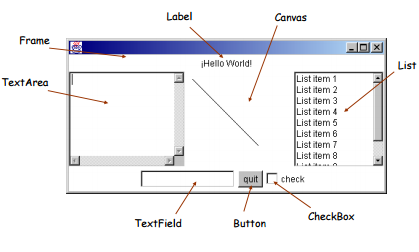
\includegraphics[scale=.7]{images/awt.png}}}
		\end{center}
	\end{frame}

    \begin{frame}
		\frametitle{Swing}
		\framesubtitle{Antes de comenzar}
		\begin{center}
            	\fbox{\fbox{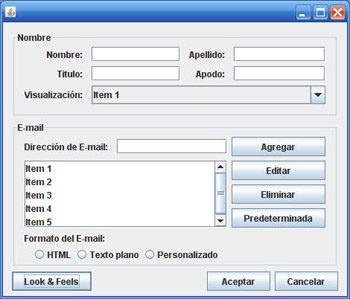
\includegraphics[scale=.8]{images/swing.png}}}
		\end{center}
	\end{frame}

    \section{Caracter\'isticas}
    
	\begin{frame}
		\frametitle{Swing}
		\framesubtitle{Caracter\'isticas}
		
		Algunas caracter\'isticas de Swing. 
		{\scriptsize
		\begin{itemize}
		    \item[$\rightarrow$] Paquete de Java para la generaci\'on del GUI en aplicaciones reales. 
		    \item[$\rightarrow$] Disponible como paquete externo en Java 1.1 e integrado desde Java 1.2.
		    \item[$\rightarrow$] Es una de las API de JFC (Java Foundation Classes): AWT, Java 2D, Accessibility, Drag and Drop, Swing, etc.
		    \item[$\rightarrow$] Escrito totalmente en Java. 
		    \item[$\rightarrow$] No reemplaza a AWT. (Se apoya sobre AWT y a\~nade JComponents).
		    \item[$\rightarrow$] Utiliza el modelo de eventos de Java 1.1.
		    \item[$\rightarrow$] Elecci\'on entre diferentes aspectos (look \& feel).
		    \item[$\rightarrow$] Arquitectura Model-View-Controller (MVC).
		    \item[$\rightarrow$] Nuevos componentes (\'arboles, tablas, frames internos, \'iconos, bordes, tooltips, etc).
		\end{itemize}}
	\end{frame}    
    
    \begin{frame}
		\frametitle{Swing}
		\framesubtitle{Caracter\'isticas - Jerarqu\'ia de clases}
		\begin{center}
            	\fbox{\fbox{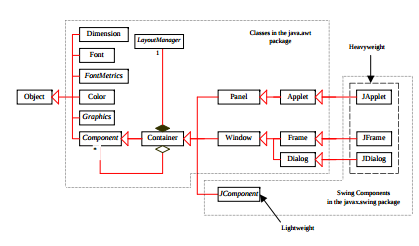
\includegraphics[scale=.7]{images/jerarquia.png}}}
		\end{center}
	\end{frame}

	\begin{frame}
		\frametitle{Swing}
		\framesubtitle{Caracter\'isticas - Jerarqu\'ia de clases}
		
		{\scriptsize
		\begin{itemize}
		    \item[$\rightarrow$] \textbf{Component}: superclase de todas las clases de interfaz gr\'afica.
		    \item[$\rightarrow$] \textbf{Container}: para agrupar componentes.
            \item[$\rightarrow$] \textbf{JComponent}: superclase de todos los componentes de \textbf{Swing}. Sus subclases son los elementos b\'asicos de la GUI.
            \item[$\rightarrow$] \textbf{JFrame}: ventana que no est\'a contenida en otras ventanas.
            \item[$\rightarrow$] \textbf{JDialog}: cuadro de di\'alogo.
            \item[$\rightarrow$] \textbf{JApplet}: subclase de Applet para crear applets tipo \textbf{Swing}.
            \item[$\rightarrow$] \textbf{JPanel}: contenedor invisible que mantiene componentes de interfaz y que se puede anidar, coloc\'andose en otros paneles o en ventanas.
            \item[$\rightarrow$] \textbf{Graphics}: clase abstracta que proporciona contextos gr\'aficos donde dibujar cadenas de texto, l\'ineas y otras formas sencillas.
            \item[$\rightarrow$] \textbf{Color}: color de los componentes gr\'aficos.
            \item[$\rightarrow$] \textbf{Font}: aspecto de los caracteres.
            \item[$\rightarrow$] \textbf{FontMetrics}: clase abstracta para propiedades de las fuentes.
		\end{itemize}}
	\end{frame}

	\begin{frame}
		\frametitle{Swing}
		\framesubtitle{Caracter\'isticas - Jerarqu\'ia de clases}
		
		Categor\'ias de clases
		\begin{itemize}
		    \item[\checkmark] Contenedores:
		    \begin{itemize}
        		    \item[$\rightarrow$] \textbf{JFrame}, JApplet, JWindow, JDialog.
        		\end{itemize}
		    \item[\checkmark] Componentes intermedios:
		    \begin{itemize}
        		    \item[$\rightarrow$] \textbf{JPanel}, JScrollPane.
        		\end{itemize}
		    \item[\checkmark] Componentes:
		    \begin{itemize}
        		    \item[$\rightarrow$] JLabel, JBbutton, JTextField, JTextArea, etc.
        		\end{itemize}
		    \item[\checkmark] Clases de soporte:
		    \begin{itemize}
        		    \item[$\rightarrow$] Graphics, Color, Font, etc.
        		\end{itemize}        		
		\end{itemize}
	\end{frame}

    \begin{frame}
		\frametitle{Swing}
		\framesubtitle{Caracter\'isticas - Jerarqu\'ia de clases}
		\begin{center}
            	\fbox{\fbox{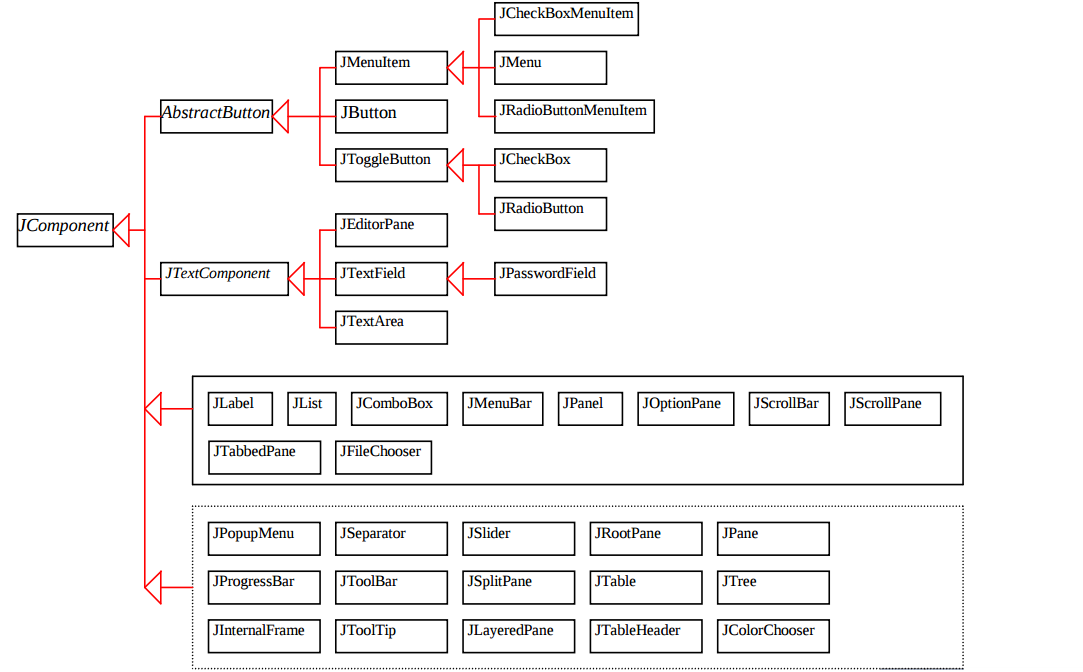
\includegraphics[scale=.25]{images/jcomponent.png}}}
		\end{center}
	\end{frame}

	\begin{frame}
		\frametitle{Swing}
		\framesubtitle{Caracter\'isticas - Jerarqu\'ia de clases}
		
		Contenedores de alto nivel: 
		\begin{itemize}
		    \item[\checkmark] \textbf{JFrame}
		    \begin{itemize}
        		    \item[$\rightarrow$] Habitualmente la clase JFrame se emplea para crear la ventana principal de una aplicaci\'on en Swing.
        		\end{itemize}
		    \item[\checkmark] \textbf{JDialog}
		    \begin{itemize}
        		    \item[$\rightarrow$] Ventanas de interacci\'on con el usuario.
        		\end{itemize}        		
		\end{itemize}
		
		Contenedores intermedios: 
		\begin{itemize}
		    \item[\checkmark] \textbf{JPanel}
		    \begin{itemize}
        		    \item[$\rightarrow$] Agrupa a otros componentes.
        		\end{itemize}
		    \item[\checkmark] \textbf{JScrollPanel}
		    \begin{itemize}
        		    \item[$\rightarrow$] Incluye barras de desplazamiento.
        		\end{itemize}        		
		\end{itemize}
	\end{frame}

    \begin{frame}
		\frametitle{Swing}
		\framesubtitle{Caracter\'isticas - Jerarqu\'ia de clases}
		\begin{center}
            	\fbox{\fbox{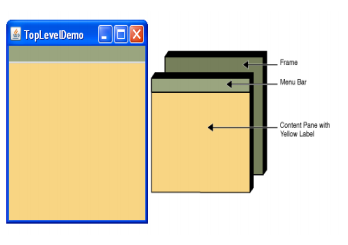
\includegraphics[scale=.7]{images/contenedores.png}}}
		\end{center}
	\end{frame}

    \begin{frame}
		\frametitle{Swing}
		\framesubtitle{Caracter\'isticas - Esquema de aplicaci\'on en Swing}
		
    		\begin{center}
            	\fbox{\fbox{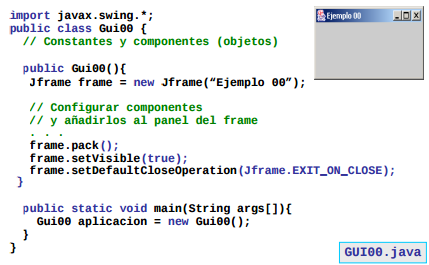
\includegraphics[scale=.68]{images/Gui00.png}}}
		\end{center}
	\end{frame}

	\begin{frame}
		\frametitle{Swing}
		\framesubtitle{Caracter\'isticas - Esquema de aplicaci\'on en Swing}
		
		Modo 1: 
		\begin{itemize}
		    \item[\checkmark] 1. Obtenemos el panel de contenido del frame:
		    \begin{itemize}
        		    \item[$\rightarrow$] \textbf{Container} panel = \textbf{this.getContentPane()};
        		\end{itemize}
		    \item[\checkmark] 2. A\~nadimos componentes a dicho panel:
		    \begin{itemize}
        		    \item[$\rightarrow$] panel.add(\emph{\textbf{unComponente}});
        		\end{itemize}        		
		\end{itemize}
		
		Modo 2:
		\begin{itemize}
		    \item[\checkmark] A partir de 1.5 tambi\'en se puede hacer directamente sobre el Jframe:
		    \begin{itemize}
        		    \item[$\rightarrow$] add(\emph{\textbf{unComponente}});
        		\end{itemize}
		\end{itemize}
	\end{frame}

    \begin{frame}
		\frametitle{Swing}
		\framesubtitle{Caracter\'isticas - Esquema de aplicaci\'on en Swing}
		
    		\begin{center}
            	\fbox{\fbox{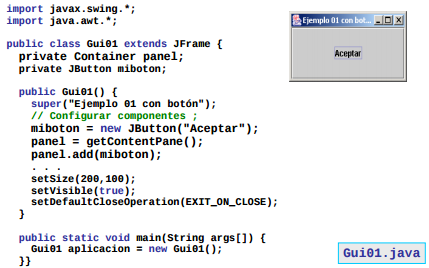
\includegraphics[scale=.68]{images/Gui01.png}}}
		\end{center}
	\end{frame}
	
    \begin{frame}
		\frametitle{Swing}
		\framesubtitle{Caracter\'isticas - Esquema de aplicaci\'on en Swing}

		\textbf{Resolver combinaciones}.
		\begin{itemize}
		    \item[\checkmark] 1. Con herencia de JFrame utilizando Container.
		    \item[?] 2. Con herencia de JFrame sin Container.
		    \item[?] 3. Sin herencia de JFrame con Container.
		    \item[?] 4. Sin herencia de JFrame sin Container.
		\end{itemize}
	\end{frame}	
	
    \begin{frame}
		\frametitle{Swing}
		\framesubtitle{Caracter\'isticas - Administradores de disposici\'on}

		\begin{itemize}
		    \item[$\rightarrow$] Los componentes se agregan al contenedor con el m\'etodo \textbf{add}().
		    \item[] \textbf{JButton} unBoton = new \textbf{JButton}("Texto del bot\'on");
		    \item[] panel.add(unBoton);
            \item[$\rightarrow$] El efecto de \textbf{add}() depende del esquema de colocaci\'on o disposici\'on (layout) del contenedor que se use.
        \end{itemize}
        
        \begin{itemize}
            \item[$\rightarrow$] Existen diversos esquemas de disposici\'on: \textbf{FlowLayout}, \textbf{BorderLayout}, \textbf{GridLayout}, etc.
            \item[$\rightarrow$] Los objetos contenedores se apoyan en objetos \textbf{LayoutManager} (administradores de disposici\'on).
            \item[$\rightarrow$] Clases m\'as usadas que implementa la interfaz LayoutManager: 
            \begin{itemize}
    		        \item[\checkmark] \textbf{FlowLayout}: un componente tras otro de izquierda a derecha.
                \item[\checkmark] \textbf{BorderLayout}: 5 regiones en el contenedor (North, South, Center, West \& Est).
                \item[\checkmark] \textbf{GridLayout}: contenedor en filas y columnas (grilla).
            \end{itemize}
		\end{itemize}
	\end{frame}		
	
    \begin{frame}
		\frametitle{Swing}
		\framesubtitle{Caracter\'isticas - Administradores de disposici\'on}

		\begin{itemize}
		    \item[$\rightarrow$] Para organizar el contenedor se utiliza el m\'etodo \textbf{setLayout}():
		    \item[] \textbf{public} \textbf{void} \textbf{setLayout}(\textbf{LayoutManager} mgr)
		    \item[] 
		    \item[$\rightarrow$] \textbf{setLayout}(new \textbf{BorderLayout}());
		    \item[$\rightarrow$] \textbf{setLayout}(new \textbf{FlowLayout}());
		    \item[$\rightarrow$] \textbf{setLayout}(new \textbf{GridLayout}(3,4));
		    \item[] 
		    \item[\checkmark] El layout manager elige la mejor posici\'on y tama\~no de cada componente de acuerdo al espacio disponible.
        \end{itemize}
	\end{frame}
	
	\begin{frame}
		\frametitle{Swing}
		\framesubtitle{Caracter\'isticas - Administradores de disposici\'on}

		\begin{multicols}{2}
		    \begin{center}
		        \textbf{BorderLayout} organiza el contenedor en 5 zonas. Cada zona se organiza en FlowLayout:
		        	\fbox{\fbox{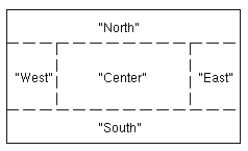
\includegraphics[scale=.55]{images/border.png}}}
		    \end{center}
		    \begin{center}
		        \textbf{FlowLayout} organiza los componentes de izquierda a derecha y de arriba hacia abajo:
		        	\fbox{\fbox{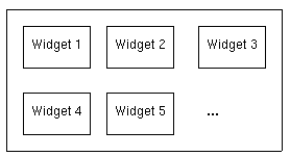
\includegraphics[scale=.52]{images/flow.png}}}
		    \end{center}
		\end{multicols}
	\end{frame}
	
	\begin{frame}
		\frametitle{Swing}
		\framesubtitle{Caracter\'isticas - Administradores de disposici\'on - Flow}

	    \begin{center}
	        	\fbox{\fbox{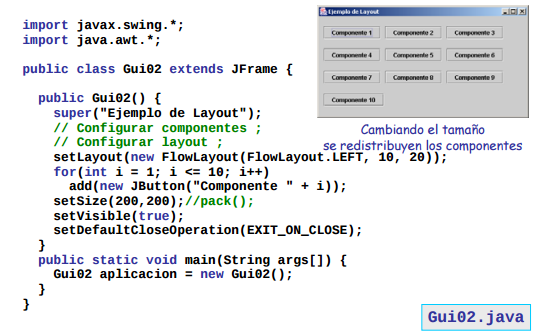
\includegraphics[scale=.52]{images/flow-code.png}}}
	    \end{center}
	\end{frame}	
	
	\begin{frame}
		\frametitle{Swing}
		\framesubtitle{Caracter\'isticas - Administradores de disposici\'on - Border}

	    \begin{center}
	        	\fbox{\fbox{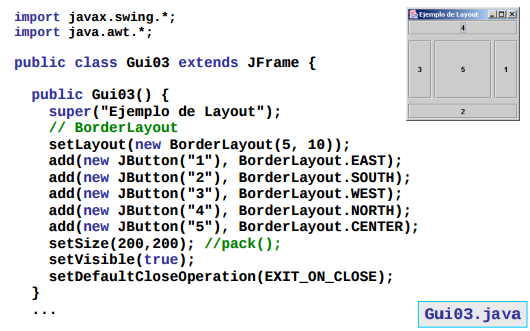
\includegraphics[scale=.52]{images/border-code.png}}}
	    \end{center}
	\end{frame}		
	
	\begin{frame}
		\frametitle{Swing}
		\framesubtitle{Caracter\'isticas - Administradores de disposici\'on - Grid}

	    \begin{itemize}
		    \item[$\rightarrow$] Crea una zona de \textbf{filas} $\times$ \textbf{columnas} componentes y \'estos se van acomodando de izquierda a derecha y de arriba a abajo. 
		    \item[$\rightarrow$] \textbf{GridLayout} tiene otro constructor que permite establecer la separaci\'on (en pixels) ente los componentes, que es cero con el primer constructor.
		    \item[] As\'i, por ejemplo:
            	    \begin{itemize}
		    		    \item[] \textbf{new} \textbf{GridLayout}(3, 4, 2, 2);
		    	    \end{itemize}
		    \item[$\rightarrow$] crea una organizaci\'on de 3 filas y 4 columnas donde los componentes quedan a dos pixels de separaci\'on.
        \end{itemize}
	\end{frame}		
	
	\begin{frame}
		\frametitle{Swing}
		\framesubtitle{Caracter\'isticas - Administradores de disposici\'on - Grid}

	    \begin{center}
	        	\fbox{\fbox{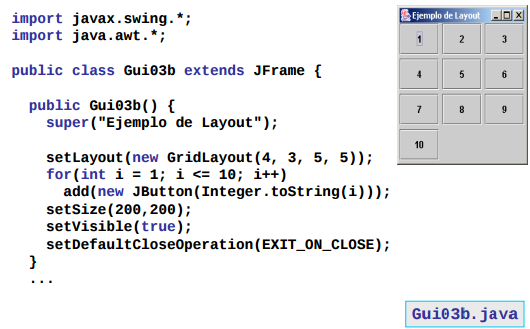
\includegraphics[scale=.52]{images/grid-code.png}}}
	    \end{center}
	\end{frame}		
	
	
	\begin{frame}
		\frametitle{Swing}
		\framesubtitle{Caracter\'isticas - Paneles como contenedores}

        Los paneles act\'uan como peque\~nos contenedores para agrupar componentes. Colocamos los componentes en paneles y los paneles en el frame o incluso en otros paneles.

	    \begin{center}
	        	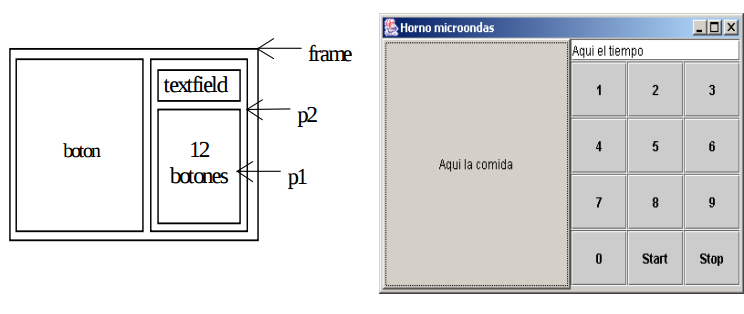
\includegraphics[scale=.37]{images/panel-container.png}
	    \end{center}
	\end{frame}			
	
	\begin{frame}
		\frametitle{Swing}
		\framesubtitle{Caracter\'isticas - Ejercicio}

        Desarrolle \textbf{s\'olo} la interfaz gr\'afica de usuario de una calculadora b\'asica.

	    \begin{center}
	        	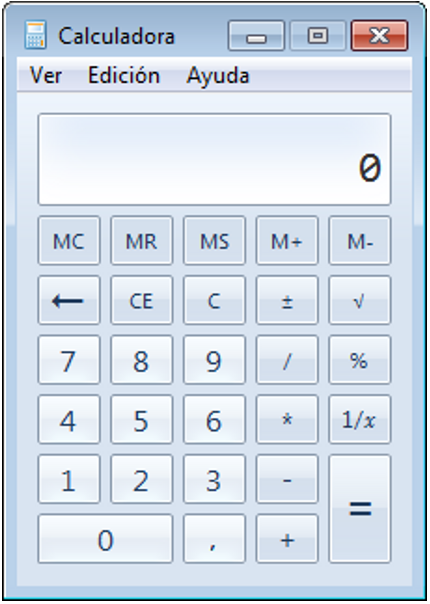
\includegraphics[scale=.35]{images/calculadora.png}
	    \end{center}
	\end{frame}		
	
{ % all template changes are local to this group.
    \usebackgroundtemplate{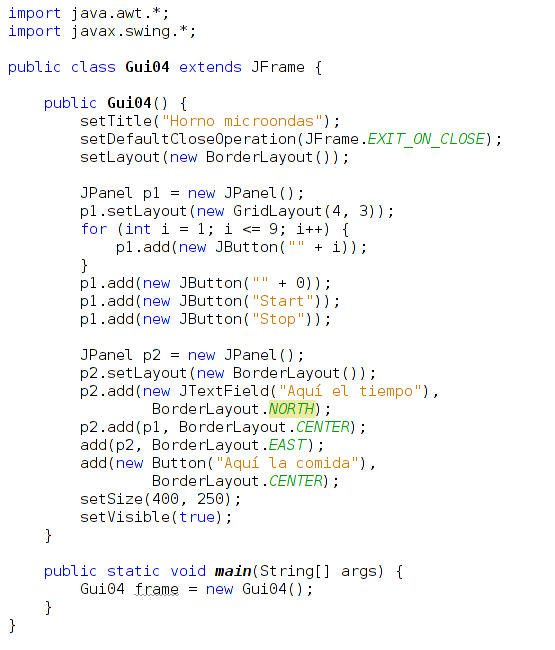
\includegraphics[scale=.425]{images/Gui04.png}}
    \setbeamertemplate{navigation symbols}{}
    \begin{frame}[plain]
    \end{frame}
}

	\begin{frame}
		\frametitle{Swing}
		\framesubtitle{Caracter\'isticas - Intereacci\'on con el usuario}

        Al interactuar con la aplicaci\'on, el usuario:

	    \begin{itemize}
		    \item[$\rightarrow$] Acciona componentes (\textbf{ActionEvent}).
		    \item[] El usuario pulsa un bot\'on. 
		    \item[] El usuario termina de introducir un texto en un campo y presiona Enter. 
		    \item[] El usuario selecciona un elemento de una lista pulsando el preferido (o de un men\'u).
		    \item[] Pulsa o suelta botones del rat\'on (\textbf{MouseEvent}).
		    \item[$\rightarrow$] Minimiza, cierra o manipula una ventana (\textbf{WindowEvent}).
		    \item[$\rightarrow$] Escribe con el teclado (\textbf{KeyEvent}).
		    \item[$\rightarrow$] Descubre porciones de ventanas (\textbf{PaintEvent}).
        \end{itemize}
	\end{frame}	

	\begin{frame}
		\frametitle{Swing}
		\framesubtitle{Caracter\'isticas - Intereacci\'on con el usuario}

        Al interactuar con la aplicaci\'on, el usuario:

	    \begin{itemize}
		    \item[] Cuando el usuario de un programa mueve el rat\'on, cambia el foco o pulsa una tecla, genera un evento (actionEvent).
		    \item[] Los eventos son objetos de ciertas clases. Normalmente un objeto de alguna subclase de \textbf{EventObject} que indica:
		    \begin{itemize}
        		    \item[\checkmark] El elemento que accion\'o el usuario.
        		    \item[\checkmark] La identificaci\'on del evento que indica su naturaleza.
        		    \item[\checkmark] La posici\'on del rat\'on en el momento de la interacci\'on.
        		    \item[\checkmark] Teclas adicionales pulsadas por el usuario, como la tecla \emph{Control}, la tecla de cambio a may\'usculas (\emph{shift}), etc.
	    	    \end{itemize}
        \end{itemize}
	\end{frame}	

	\begin{frame}
		\frametitle{Swing}
		\framesubtitle{Caracter\'isticas - Intereacci\'on con el usuario - Acciones}
        {\scriptsize
        \begin{tabular}{p{6cm}p{2.5cm}p{2.5cm}} \hline 
            \textbf{Acci\'on} & \textbf{Objeto origen} & \textbf{Tipo de evento} \\ \hline
            \multirow{2}{*}{Pulsar un bot\'on} & \multirow{2}{*}{JButton} & \multirow{2}{*}{ActionEvent} \\ & & \\ \hline
            \multirow{2}{*}{Cambio del texto} & \multirow{2}{*}{JTextComponent} & \multirow{2}{*}{TextEvent} \\ & & \\ \hline
            \multirow{2}{*}{Pulsar Enter/Intro en un campo de texto} & \multirow{2}{*}{JTextField} & \multirow{2}{*}{ActionEvent} \\ & & \\ \hline
            \multirow{2}{*}{Selecci\'on de un nuevo elemento} & \multirow{2}{*}{JCombobox} & ItemEvent \\
            & & ActionEvent \\ \hline
            \multirow{2}{*}{Selecci\'on de elemento(s)} & \multirow{2}{*}{JList} & \multirow{2}{*}{ListSelectionEvent} \\ & & \\ \hline
            \multirow{2}{*}{Pulsar una casilla de verificaci\'on} & \multirow{2}{*}{JCheckBox} & ItemEvent \\
            & & ActionEvent \\ \hline
            \multirow{2}{*}{Pulsar un bot\'on de radio} & \multirow{2}{*}{JRadioButton} & ItemEvent \\
            & & ActionEvent \\ \hline
            \multirow{2}{*}{Selecci\'on de una opci\'on de men\'u} & \multirow{2}{*}{JMenuItem} & \multirow{2}{*}{ActionEvent} \\ & & \\ \hline
            \multirow{2}{*}{Mover la barra de desplazamiento} & \multirow{2}{*}{JScrollBar} & \multirow{2}{*}{AdjustmentEvent} \\ & & \\ \hline
            \multirow{2}{*}{Abrir, minimizar, maximizar o cerrar la ventana} & \multirow{2}{*}{JWindow} & \multirow{2}{*}{WindowEvent} \\ & &\\ \hline
        \end{tabular}}
	\end{frame}	

	\begin{frame}
		\frametitle{Swing}
		\framesubtitle{Caracter\'isticas - Intereacci\'on con el usuario - Ejemplo}
        
        Al pulsar el bot\'on Copiar, se debe copiar el valor del cuadro ''Valor'' en el cuadro ''Copia''.
        \begin{center}
	        	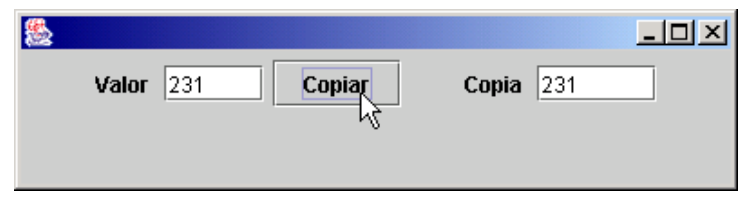
\includegraphics[scale=.35]{images/copia.png}
	    \end{center}
	\end{frame}	

{ % all template changes are local to this group.
    \usebackgroundtemplate{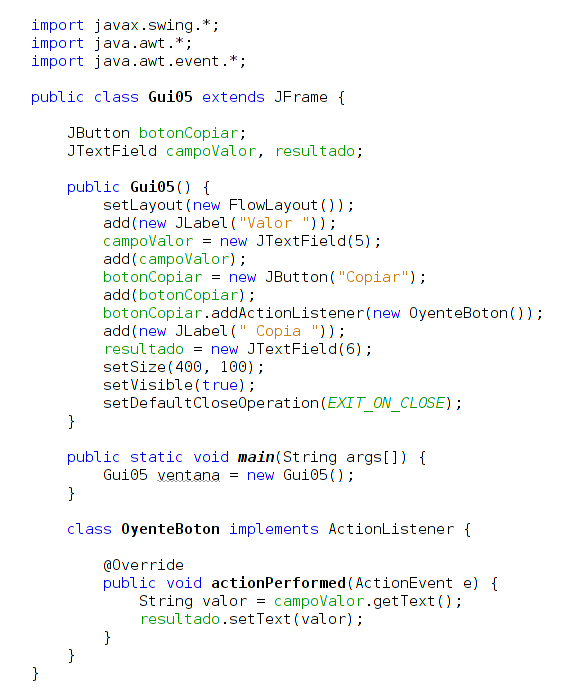
\includegraphics[scale=.4]{images/Gui05.png}}
    \setbeamertemplate{navigation symbols}{}
    \begin{frame}[plain]
    \end{frame}
}

	\begin{frame}
		\frametitle{Swing}
		\framesubtitle{Caracter\'isticas - Intereacci\'on con el usuario - Ejemplo}

        Cambiar el color del panel mediante eventos de bot\'on.
        \begin{center}
	        	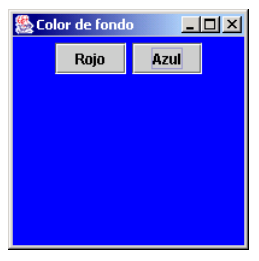
\includegraphics[scale=.45]{images/colores.png}
	    \end{center}
	\end{frame}	

{ % all template changes are local to this group.
    \usebackgroundtemplate{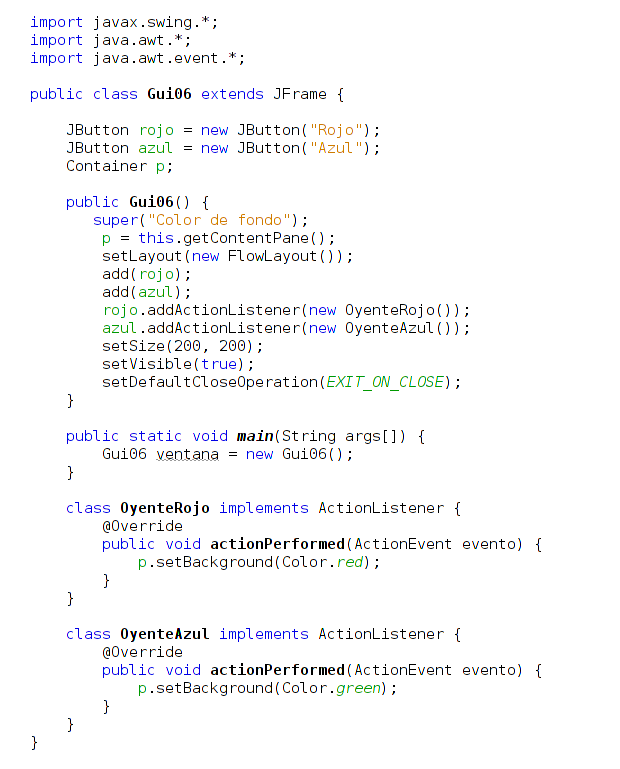
\includegraphics[scale=.35]{images/Gui06.png}}
    \setbeamertemplate{navigation symbols}{}
    \begin{frame}[plain]
    \end{frame}
}

    \begin{frame}
		\frametitle{Swing}
		\framesubtitle{Componentes}

        \begin{itemize}
		    \item[\checkmark] \textbf{JButton}: Bot\'on aislado. Puede pulsarse, pero su estado no cambia.
		    \item[\checkmark] \textbf{JToggleButton}: Bot\'on seleccionable. Cuando se pulsa el bot\'on, su estado pasa a seleccionado, hasta que se pulsa de nuevo (entonces se deselecciona)
		    \begin{itemize}
        		    \item[] \textbf{isSelected}() permite chequear su estado.
	    	    \end{itemize}
		    \item[\checkmark] \textbf{JCheckBox}: Especializaci\'on de \emph{JToggleButton} que implementa una casilla de verificaci\'on. Bot\'on con estado interno, que cambia de apariencia de forma adecuada seg\'un si est\'a o no est\'a seleccionado
		    \item[\checkmark] \textbf{JRadioButton}: Especializaci\'on de \emph{JToggleButton} que tiene sentido dentro de un mismo grupo de botones (ButtonGroup) que controla que s\'olamente uno de ellos est\'a seleccionado.
		\end{itemize}
	\end{frame}	

    \begin{frame}
		\frametitle{Swing}
		\framesubtitle{Componentes - JButton}

        \begin{itemize}
		    \item[\checkmark] Constructores:
		    \begin{itemize}
        		    \item[] \textbf{JButton}(String text)
        		    \item[] \textbf{JButton}(Icon icon)
        		    \item[] \textbf{JButton}(String text, Icon icon)
	    	    \end{itemize}
		\end{itemize}

        \begin{itemize}
		    \item[\checkmark] Respuesta a botones:
		    \begin{itemize}
        		    \item[] Implementar la interfaz \textbf{ActionListener}.
        		    \item[] Implementar el m\'etodo \textbf{actionPerformed}(\textbf{ActionEvent} e).
	    	    \end{itemize}
		\end{itemize}
	\end{frame}	
	
	\begin{frame}
		\frametitle{Swing}
		\framesubtitle{Componentes - JButton}

        \begin{center}
	        	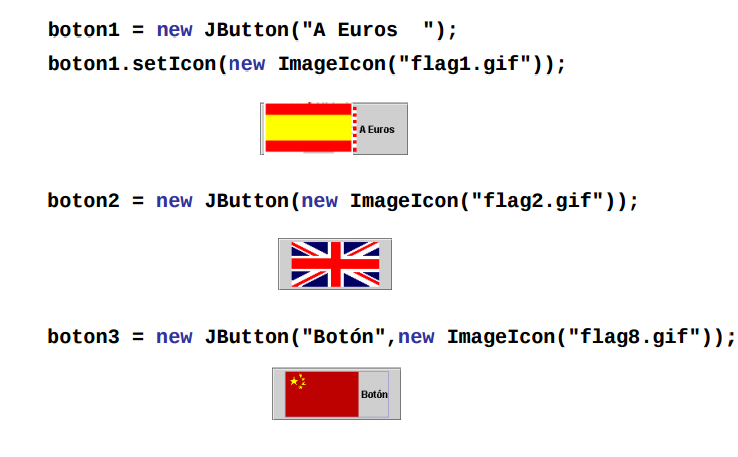
\includegraphics[scale=.45]{images/ejemplo-jbutton.png}
	    \end{center}
	\end{frame}		

    \begin{frame}
		\frametitle{Swing}
		\framesubtitle{Componentes - JLabel}

        \begin{itemize}
		    \item[\checkmark] Para texto, una imagen o ambos:
		    \begin{itemize}
        		    \item[] \textbf{JLabel}(String text, int horizontalAlignment)
        		    \item[] \textbf{JLabel}(String text)
        		    \item[] \textbf{JLabel}(Icon icon)
        		    \item[] \textbf{JLabel}(Icon icon, int horizontalAlignment)
	    	    \end{itemize}
		\end{itemize}
	\end{frame}	

    \begin{frame}
		\frametitle{Swing}
		\framesubtitle{Componentes - JLabel}

        \begin{center}
	        	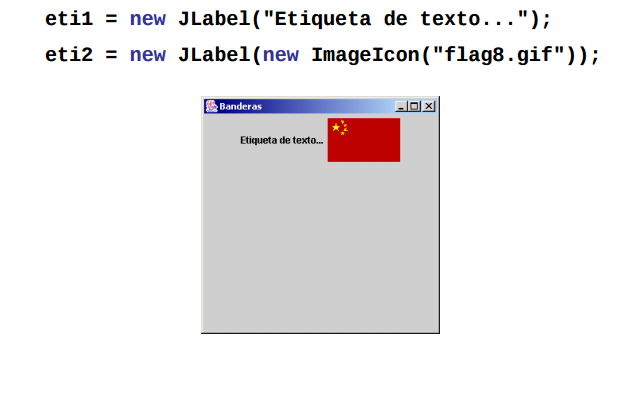
\includegraphics[scale=.45]{images/ejemplo-jlabel.png}
	    \end{center}
	\end{frame}	

    \begin{frame}
		\frametitle{Swing}
		\framesubtitle{Componentes - JLabel}

        \begin{itemize}
		    \item[\checkmark] Campos de texto para introducir caracteres:
		    \begin{itemize}
        		    \item[] \textbf{JTextField}(int columns)
        		    \item[] \textbf{JTextField}(String text)
        		    \item[] \textbf{JTextField}(String text, int columns)
        		    \item[] \textbf{JTextField} text1 = new JTextField(''hola'', 10);
	    	    \end{itemize}
	    	    \item[$\rightarrow$] Fijar texto: text1.setText(''Adios'');
	    	    \item[$\rightarrow$] Obtener texto: String str = text1.getText();
	    	    \item[$\rightarrow$] Agregar al Panel: p1.add(text1);
		\end{itemize}
	\end{frame}	

    \begin{frame}
		\frametitle{Swing}
		\framesubtitle{Componentes - JComboBox}

        \begin{itemize}
		    \item[\checkmark] Listas de elementos para seleccionar un \'unico valor:
		    \begin{itemize}
        		    \item[] Creaci\'on: \textbf{JComboBox} ch1 = \textbf{new} \textbf{JComboBox}();
        		    \item[] Agregar opciones: ch1.\textbf{addItem}(Object elemento);
        		    \item[] Registrar Evento: ch1.\textbf{addItemListener}(objeto\_oyente);
        		    \item[] Obtener selecci\'on: \textbf{String} val = (\textbf{String}) ch1.\textbf{getSelectedItem}();
	    	    \end{itemize}
	    	    \item[$\rightarrow$] Implementar la interfaz \textbf{ItemListener}.
	    	    \item[$\rightarrow$] Implementar el m\'etodo \textbf{itemStateChanged}(ItemEvent e)
	    	    \item[] \textbf{class OyenteItem implements} ItemListener \{
	    	    \item[] \hspace{10pt} \textbf{public void} itemStateChanged(\textbf{ItemEvent} e) \{
            \item[] \hspace{10pt} ...	    	    
            \item[] \hspace{10pt}\}
            \item[] \}
		\end{itemize}
        
	\end{frame}	

    \begin{frame}
		\frametitle{Swing}
		\framesubtitle{Componentes - JList}

        \begin{itemize}
		    \item[\checkmark] Implementar la interfaz \textbf{ListSelectionListenner}
		    \item[\checkmark] Implementar el m\'etodo \textbf{valueChanged}(ListSelectionEvent e)
		    \begin{itemize}
        		    \item[] l.\textbf{addListSelectionListener}(new \textbf{OyenteLista}());
	    	        \item[] ...
    	    	        \item[] \textbf{class OyenteLista implements} ListSelectionListener \{
	    	        \item[] \hspace{10pt} \textbf{public void} valueChanged(\textbf{ListSelectionEvent} e) \{
	    	        \item[] \hspace{20pt} \textbf{int}[] indices = l.\textbf{getSelectedIndices}();
	    	        \item[] \hspace{20pt} \textbf{int} i;
	    	        \item[] \hspace{20pt} \textbf{for}(\textbf{int} i = 0; i $<$ indices.length; i++) \{
                \item[] \hspace{30pt} ...
                \item[] \hspace{20pt} \}
                \item[] \hspace{10pt} \}
                \item[] \}   
            \end{itemize}
		\end{itemize}
	\end{frame}	

    \begin{frame}
		\frametitle{Swing}
		\framesubtitle{Componentes - Interacci\'on modal}

        \begin{center}
	        	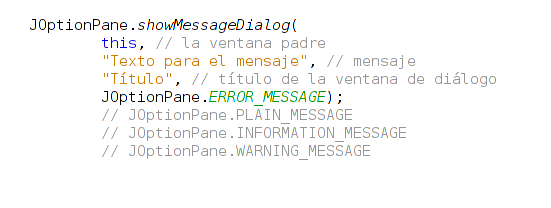
\includegraphics[scale=.7]{images/dialog.png}
	    \end{center}
	\end{frame}	

{ % all template changes are local to this group.
    \usebackgroundtemplate{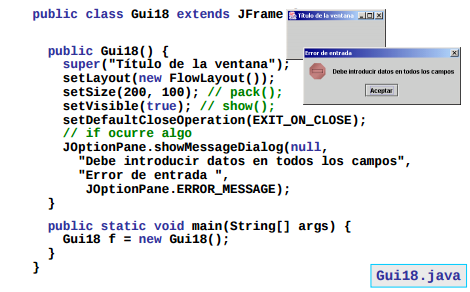
\includegraphics[scale=.75]{images/Gui18.png}}
    \setbeamertemplate{navigation symbols}{}
    \begin{frame}[plain]
    \end{frame}
}

{ % all template changes are local to this group.
    \usebackgroundtemplate{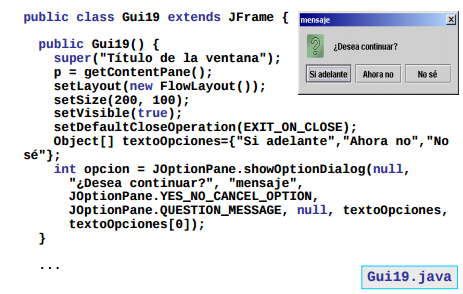
\includegraphics[scale=.75]{images/Gui19.png}}
    \setbeamertemplate{navigation symbols}{}
    \begin{frame}[plain]
    \end{frame}
}

{ % all template changes are local to this group.
    \usebackgroundtemplate{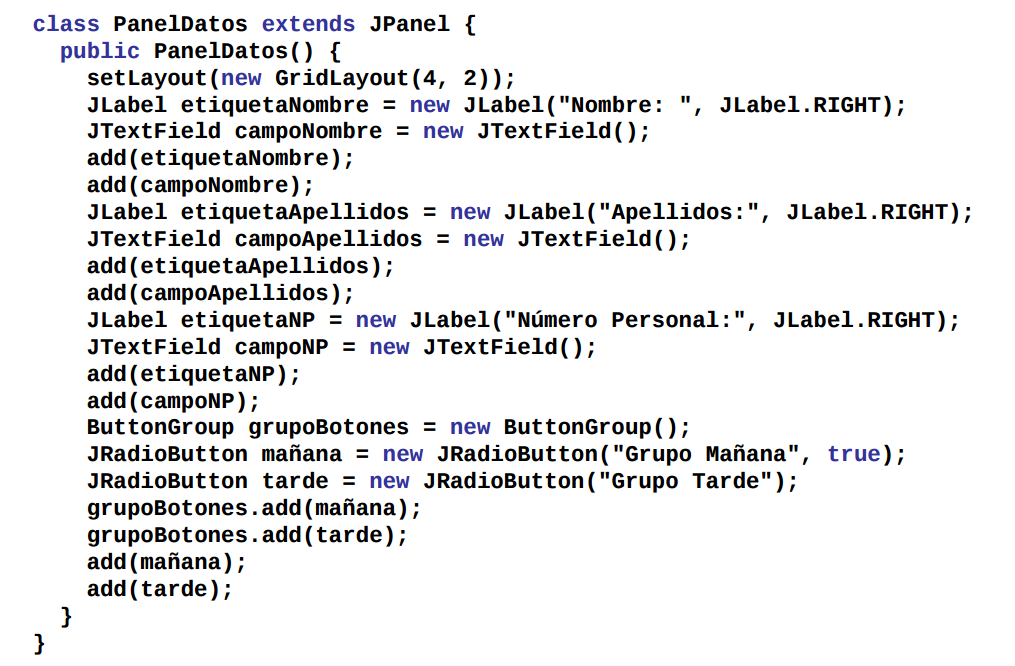
\includegraphics[scale=.35]{images/panel-datos.png}}
    \setbeamertemplate{navigation symbols}{}
    \begin{frame}[plain]
    \end{frame}
}

{ % all template changes are local to this group.
    \usebackgroundtemplate{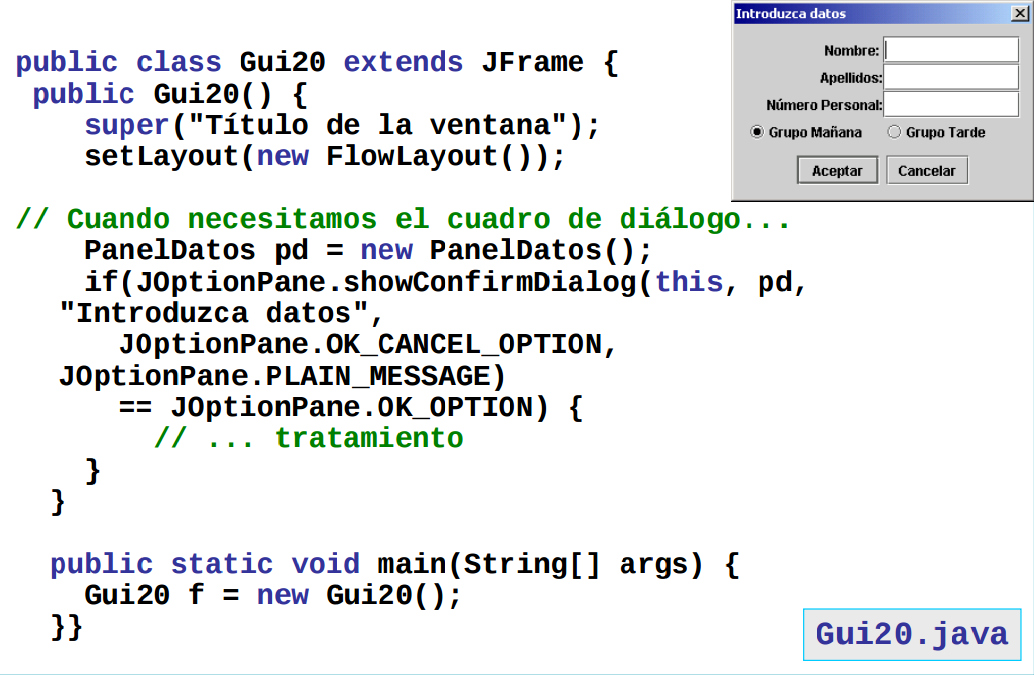
\includegraphics[scale=.35]{images/Gui20.png}}
    \setbeamertemplate{navigation symbols}{}
    \begin{frame}[plain]
    \end{frame}
}

    \begin{frame}
		\frametitle{Preguntas}

		\hspace{4cm}\huge{Preguntas ?}
		
	\end{frame}
	
    \begin{frame}
		\frametitle{Tarea}
        \framesubtitle{Transformaci\'on N\'umeros Romanos}
        {\scriptsize
        El sistema de numeraci\'on romana se desarroll\'o en la antigua Roma y se utiliz\'o en todo su imperio. Es un sistema de numeraci\'on no posicional, en el que se usan algunas letras may\'usculas como s\'imbolos para representar los n\'umeros. 
        \vspace{1pt}
        La siguiente tabla muestra los s\'imbolos v\'alidos en el sistema de numeraci\'on romano, y sus equivalencias en el sistema decimal:
		\vspace{1pt}
	    
	    \begin{center}
		\begin{tabular}{|c|c|c|} \hline
			\multicolumn{1}{|>{\columncolor[rgb]{0.8, 0.8, 0.8}}c|}{\textbf{Romano}} &
			\multicolumn{1}{|>{\columncolor[rgb]{0.8, 0.8, 0.8}}c|}{\textbf{Decimal}} &
			\multicolumn{1}{|>{\columncolor[rgb]{0.8, 0.8, 0.8}}c|}{\textbf{Nota}} \\ \hline
			I	& 1 		& Unus \\ \hline
			V	& 5 		& Quinque \\ \hline
			X	& 10		& Decem \\ \hline
			L	& 50		& Quinquaginta \\ \hline
			C	& 100	& Centum \\ \hline
			D	& 500	& Quingenti \\ \hline
			M	& 1000	& Mille \\ \hline
		\end{tabular}
		\end{center}}
	\end{frame}
	
    \begin{frame}
		\frametitle{Tarea}
        \framesubtitle{Transformaci\'on N\'umeros Romanos}
        {\scriptsize
        Desarrolle un programa con interfaz de usuario que convierta un entero positivo (ingresado en un campo de texto), en un n\'umero romano. Las reglas para construir un n\'umero romano son las siguentes:
        
		\begin{itemize}
			\item[$\rightarrow$] Los s\'imbolos con un valor grande usualmente aparecen antes que los con menor valor.
			\item[$\rightarrow$] El valor de un n\'umero romano es, en general, la suma de los valores de los s\'imbolos. Por ejemplo, II es 2, VIII es 8. 
			\item[$\rightarrow$] Si un s\'imbolo de menor valor aparece antes de uno de mayor valor, el valor de los dos s\'imbolos es la diferencia entre ambos. Por ejemplo, IV es 4, IX es 9, y LIX es 59.
			\item[$\rightarrow$] Note que no hay cuatro s\'imbolos consecutivos iguales. Por ejemplo, IV, pero no IIII, es el n\'umero 4.
			\item[$\rightarrow$] Los n\'umeros romanos construidos de esta forma pueden no ser \'unicos. Por ejemplo, MCMXC y MXM son v\'alidos para 1990. Aunque el n\'umero romano generado por su programa no debe necesariamente ser el m\'as corto, \textbf{nunca} use VV para 10, VVV para 15, LL para 100, DD para 1000, etc.
		\end{itemize}}
	\end{frame}	
	
	
\end{document}

\usetheme{default}
\usetheme{JuanLesPins}
\usetheme{Goettingen}
\usetheme{Szeged}
\usetheme{Warsaw}

\usecolortheme{crane}

\usefonttheme{serif}
\usefonttheme{structuresmallcapsserif}